\scanpage{67}\mspage{66}
% The two raised additions and their drawn connecting enclosures.
\figure{
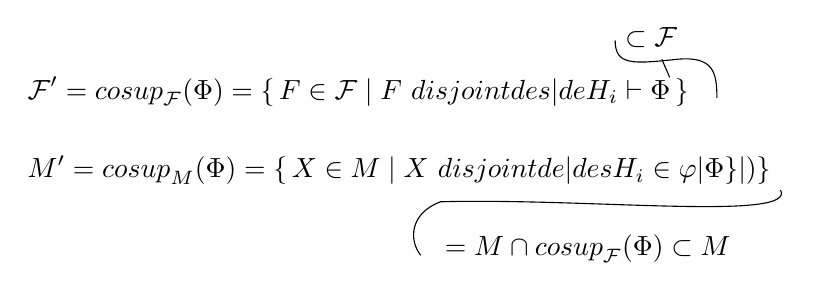
\begin{tikzpicture}[x=1cm,y=1cm,every node/.style={inner sep=0pt}]
  \node[anchor=west] (top) at (0,0) {$\displaystyle
    \mathcal F'=\operatorname{cosup}_{\mathcal F}(\Phi)
    =\{\,F\in\mathcal F\mid F\ \text{disjoint \unsure{des|de} }H_i\vdash\Phi\,\}$};
  \node[anchor=south east] (addition) at ([xshift=-.15cm,yshift=.55cm]top.east)
    {$\inserted{\subset\mathcal F}$};
  \draw ([xshift=-.12cm,yshift=.1cm]addition.south west)
    .. controls ([xshift=-.12cm,yshift=-.22cm]addition.south west)
    and ([xshift=.1cm,yshift=-.2cm]addition.south west)
    .. ([yshift=-.14cm]addition.south east)
    .. controls ([xshift=.45cm,yshift=-.1cm]addition.south east)
    and ([xshift=.35cm,yshift=.25cm]top.east)
    .. ([xshift=.35cm,yshift=-.08cm]top.east);
  \draw ([xshift=-.2cm,yshift=-.14cm]addition.south east)
    -- ([xshift=-.25cm,yshift=.18cm]top.east);
  \node[anchor=west] (second) at (0,-1) {$\displaystyle
    M'=\operatorname{cosup}_{M}(\Phi)
    =\{\,X\in M\mid X\ \text{disjoint \unsure{de|des} }H_i\in
    \unsure{\varphi|\Phi}\unsure{\rbrace|)\rbrace}$};
  \node[anchor=west] (third) at (5.3,-2) {$\displaystyle
    \inserted{=M\cap\operatorname{cosup}_{\mathcal F}(\Phi)\subset M}$};
  \draw ([xshift=.12cm,yshift=-.25cm]second.east)
    .. controls ([xshift=.33cm,yshift=-.65cm]second.east)
    and ([xshift=-1.8cm,yshift=.65cm]third.east)
    .. ([xshift=-.05cm,yshift=.6cm]third.west)
    .. controls ([xshift=-.45cm,yshift=.45cm]third.west)
    and ([xshift=-.45cm,yshift=.1cm]third.west)
    .. ([xshift=-.3cm,yshift=-.08cm]third.west);
\end{tikzpicture}}

\deleted{Donc \unsure{on aura|on a}, pour $F\in\mathcal F$ posant $\mathcal F'=\operatorname{cosup}_{\mathcal F}$,}

\[
\begin{aligned}
&\deleted{\unsure{\phi|\Phi}}\qquad
\deleted{\mathcal F'=\operatorname{cosupp}_{\mathcal F}(\Phi),\quad M'=\mathcal F'\cap M,}\\[-2pt]
&\qquad\deleted{F\in\operatorname{cosup}_{\unsure{,|\mathcal F}}}
\qquad\qquad\deleted{=\operatorname{cosup}_{\deleted{\unsure{\mathcal F}}M}(\mathcal F)}
\end{aligned}
\]

Donc pour $F\in\mathcal F$

% Left note slanted; the right notes and their enclosure are in the same group.
\figure{
\begin{tikzpicture}[x=1cm,y=1cm,every node/.style={inner sep=0pt}]
  \node[anchor=west] (pair) at (4,0) {$\displaystyle
  \left\{\begin{aligned}
  F\in\mathcal F'&\Longleftrightarrow\overline F\subset M'\\
  M'&=.\mathcal F'\cap M
  \end{aligned}\right.$};
  \node[anchor=east,align=left,rotate=17] (leftnote) at (3.5,-.2)
    {Ainsi, $M'$ et $\mathcal F'$\\
     se \unsure{déterminent|determinent}\\
     \unsure{mutuellement}};
  \node[anchor=east] at ([xshift=-.12cm,yshift=.12cm]pair.west)
    {$\unsure{\longrightarrow}$};
  \node[anchor=north west,align=left] (nb) at (12.2,1.2)
    {NB $\mathcal F',M'$\\sont des\\parties\\fermées de\\$\mathcal F,M$.};
  \node[anchor=west] (family) at (10.7,-.65) {$\mathcal F'$};
  \node[anchor=west] (stable) at (10.8,-1.35) {\uline{Stable par Sup.}};
  \draw ([xshift=-.04cm,yshift=-.15cm]family.south west)
    -- ([xshift=.32cm,yshift=-.15cm]family.south east)
    -- ([xshift=.32cm,yshift=.22cm]family.south east);
  \draw (9.3,-.95) .. controls (10.3,-.83) and (10.55,-.86) .. (10.62,-1.22)
    .. controls (10.63,-1.52) and (10.82,-1.55) .. (11.15,-1.55)
    -- ([xshift=.1cm,yshift=-.22cm]stable.south east)
    .. controls ([xshift=.6cm,yshift=-.5cm]stable.south east)
    and ([xshift=.65cm,yshift=-.65cm]stable.south east)
    .. ([xshift=.8cm,yshift=-.7cm]stable.south east);
\end{tikzpicture}}

Soit d'autre part
\[
\begin{aligned}
\mathcal F''&=\operatorname{cosupp}_{\mathcal F}(\mathcal F')\overset{\text{def}}{=}\operatorname{supp}_{\mathcal F}(\Phi)\\
M''&=\operatorname{cosup}_{M}(\mathcal F')\overset{\text{def}}{=}\operatorname{supp}_{M}(\Phi)
\end{aligned}
\]

On a \unsure{vu|bien|la|là} $\mathcal F''\supset\Phi$, $\mathcal F''$ stable par \unsure{Sup|Supp}, \deleted{contient $\Phi$} et par passage \unsure{à|:} une sous-figure. Soit $\deleted{\unsure{M}} \overline\Phi=\bigcup_{H_i\in\Phi}\overline H_i$, alors
\[
\begin{aligned}
\operatorname{cosup}_{\mathcal F}(\Phi)&=\operatorname{cosup}_{\mathcal F}(M_{\overline\Phi})\\
\operatorname{cosup}_{\deleted{\unsure{\mathcal F}}M}\unsure{\ldotp\ldotp|:}(\Phi)&=\{\,\deleted{\unsure{\varnothing|x}}X\in M\mid X\ \text{disjoint de }\unsure{\forall|\mathrm{tt}}\ Y\in M_{\overline\Phi}\,\}
\end{aligned}
\]
donc on est ramené à des constructions dans $M$. \S

\uline{Partie saturée \inserted{$\mathcal F_0$} de} $\deleted{\unsure{M}}\mathcal F$ : égale au cosupport de son cosupport ($\text{p. r. à }\mathcal F$). Partie \unsure{saturee|saturée} \inserted{$M_0$} de $M$ : égale au cosupport de son support (dans $M$). Elles se correspondent mutuellement \unsure{par|\deleted{par}}
\[
\begin{aligned}
M_0&=\mathcal F_0\cap M\\
\mathcal F_0&=\{\,F\in\mathcal F\mid\overline F\subset M_0\,\}
\end{aligned}
\]
